\documentclass[a4paper,twoside,12pt]{article}
% Alternative Options:
%	Paper Size: a4paper / a5paper / b5paper / letterpaper / legalpaper / executivepaper
% Duplex: oneside / twoside
% Base Font Size: 10pt / 11pt / 12pt


%% Language %%%%%%%%%%%%%%%%%%%%%%%%%%%%%%%%%%%%%%%%%%%%%%%%%
\usepackage[english,french]{babel}
\usepackage[latin1]{inputenc}
\usepackage[T1]{fontenc}
\usepackage{ae}
\usepackage{algorithm} %to write pseudo-code
\usepackage{algpseudocode} %to write pseudo-code

\usepackage{lmodern} %Type1-font for non-english texts and characters

\usepackage[top=2.5cm, bottom=2cm, left=2cm, right=2cm]{geometry}
\usepackage{icomma} % Permet l'utilisation de virgule comme s�parateur d�cimal
\usepackage{url} % Package pour ne pas avoir des probl�mes avec des URL's
% Utiliser \url{}

%% Packages for Graphics & Figures %%%%%%%%%%%%%%%%%%%%%%%%%%
%\usepackage[dvips]{graphicx}
%\usepackage{color,psfrag}
\usepackage{graphicx} %%For loading graphic files
%\usepackage{subfig} %%Subfigures inside a figure
%\usepackage{tikz} %%Generate vector graphics from within LaTeX
%\usepackage{tikz-3dplot} %requires 3dplot.sty to be in same directory, or in your LaTeX installation
%\usetikzlibrary{calc} %pour faire les calculs

%\usepackage{epstopdf}

\newcommand{\HRule}{\rule{\linewidth}{0.5mm}} %Dessine la ligne horizontale

%% Please note:
%% Images can be included using \includegraphics{filename}
%% resp. using the dialog in the Insert menu.
%% 
%% The mode "LaTeX => PDF" allows the following formats:
%%   .jpg  .png  .pdf  .mps
%% 
%% The modes "LaTeX => DVI", "LaTeX => PS" und "LaTeX => PS => PDF"
%% allow the following formats:
%%   .eps  .ps  .bmp  .pict  .pntg


%% Math Packages %%%%%%%%%%%%%%%%%%%%%%%%%%%%%%%%%%%%%%%%%%%%
\usepackage{amsmath,amsfonts,amstext,amscd,bezier,amsthm,amssymb}

\newcommand{\vect}[1]{\boldsymbol{#1}}

%\newenvironment{solu}{\noindent {\bf Solution.}\small }{\hfill $\square$ \normalsize \medskip}

%\renewcommand\thesection{\arabic{section}}
%\renewcommand*\thesection{Question \arabic{section}}

\def\MYTITLE{Review on boosting algorithms}

\title{\MYTITLE}
\author{\textsc{Vu} Tuan Hung and \textsc{Do} Quoc Khanh}
\date{\today}

\usepackage{fancyhdr}

\fancyhead[L]{\slshape Tuan Hung VU and Quoc Khanh DO}%\slshape\thepage LE,RO
\fancyhead[R]{\slshape Final report}%{\slshape \leftmark}
%\fancyhead[LO]{ccc}%{\slshape \rightmark}
%\fancyfoot[LO,LE]{}%\slshape Short Course on Asymptotics
\fancyfoot[C]{\thepage}
%\fancyfoot[RO,RE]{}%\slshape 7/15/2002

\DeclareMathOperator*{\argmax}{arg\,max}
\DeclareMathOperator{\Tr}{Tr}
\DeclareMathOperator{\diag}{diag}
\newcommand{\abs}[1]{{\lvert #1 \rvert}}
\newcommand{\norm}[1]{{\lVert #1 \rVert}}

\begin{document}
\maketitle
\pagestyle{fancy}

\section{Introduction}

\section{Two-class classification}
In this first part, we present an overview on boosting methods in the two-class classification framework. From a \textsl{training} set $(\textbf{x}_i, y_i)_{i = 1,...,N}$ in which $\textbf{x}_i \in \mathcal{X}$ and $y_i \in \mathcal{Y}$, we try to construct a function $F: \mathcal{X} \rightarrow \mathcal{Y}$ so that when a new value $\textbf{x}$ is randomly introduced, we have the highest probability to predict correctly the value $y$ corresponding to this value of $\textbf{x}$. Formally, we want to minimize the probability:
\begin{align}
    \mathbb{P}_{(\textbf{x}, y)} \left( y \neq F(\textbf{x})\right) \notag
\end{align}
The variable $\textbf{x}$ is called explanatory variables ($\textbf{x}$ may be multi-variational) and $y$ is called response variable. In the two-class classification framework, $\mathcal{Y} = \{ -1, 1\}$.

\subsection{Boosting and optimization in function space}\label{boo_fun_sp}
We exploit the point of view presented in \cite{trebst} by considering this problem as an estimation and optimization in function space. Indeed, if there exists a function $F^{*}$ which minimizes the above error:
\begin{align}
    F^{*} &= arg\min\limits_{F} \mathbb{P}_{(\textbf{x},y)} (y \neq F(\textbf{x})) \notag \\
    &= arg\min\limits_{F} \mathbb{E}_{(\textbf{x}, y)} \left[ 1(y \neq F(\textbf{x}))\right] \notag
\end{align}
then we are trying to estimate $F^{*}$ by a function $\hat{F}$ through the training set $(\textbf{x}_i, y_i)_{i=1,...,N}$.

\textbf{Base classifiers.} An approach frequently employed by classification algorithms is to suppose $F^{*}$ belongs to a function class parameterized by $\theta \in \Theta$:
\begin{align}
    F^{*} \in \mathcal{Q} = \left\lbrace F(., \theta) \vert \theta \in \Theta\right\rbrace \notag
\end{align}
so that the problem of estimating $F^{*}$ becomes an optimization of the parameters on $\Theta$:
\begin{align}
    \hat{\theta} = arg\min\limits_{\theta \in \Theta} \mathbb{E}_{(\textbf{x}, y)} \left[ 1(y \neq F(\textbf{x}, \theta))\right] \notag
\end{align}
and then we will take $\hat{F} = F(., \hat{\theta}) \in \mathcal{Q}$. For example, with regression tree algorithms, we have:
\begin{align}
    \mathcal{Q} = \left\lbrace F(x, \theta) = \sum\limits_{k=1}^K \lambda_k 1(\textbf{x} \in R_k) \vert (\lambda_1,...,\lambda_K) \in \mathbb{R}^K, (R_1,...,R_K) \in \mathcal{P}_{\mathcal{X}}\right\rbrace \notag
\end{align}
in which $\theta = (\lambda_{1:K}, R_{1:K})$ and $\mathcal{P}_{\mathcal{X}}$ is the set of all partitions of $\mathcal{X}$ into $K$ disjoint subsets by hyperplans which are orthogonal to axes. Similarly for support vector machines, $K$ disjoint subsets $R_1,...,R_K$ are divided by hyperplans in the reproducing kernel Hilbert space of $\mathcal{X}$ corresponding to some kernel.

We can see that a classifier is characterized by its function sub-space $\mathcal{Q}$ and the corresponding parameter space. Having the base classifiers $\mathcal{Q}_{1:M}$ with parameter spaces $\Theta_{1:M}$, instead of considering each of these classifiers separately, boosting methods consider functions of the following additive form:
\begin{align}
    \hat{F} \in \mathcal{F}_{\mathcal{Q}_1,...,\mathcal{Q}_M} = \left\lbrace \sum\limits_{m=1}^M \beta_m f(., \theta_m) \vert \theta_m \in \Theta_m, \forall m = 1,...,M\right\rbrace \notag
\end{align}
so that the optimization problem becomes:
\begin{align}
    \left\lbrace \hat{\beta}_{1:M}, \hat{\theta}_{1:M}\right\rbrace = arg\min\limits_{\beta \in \mathbb{R}^M, \theta_{1:M} \in \Theta_{1:M}} \mathbb{E}_{(\textbf{x}, y)} \left[ 1(y \neq F(\textbf{x}; \beta_{1:M}, \theta_{1:M}))\right] \label{opt_add}
\end{align}

Friedman, J. and Hastie, T. in \cite{boost} explained boosting as a forward stepwise algorithm for resolve the optimization problem \eqref{opt_add}. Friedman, J. in \cite{trebst} considered boosting like optimization algorithm in function space. We will try to adopt the latter to explain all mentioned boosting algorithms. Before going into greater details, we remark that as an classification algorithm, the boosting algorithm has its corresponding function subset which is $\mathcal{F} = \mathcal{F}_{\mathcal{Q}_1,...,\mathcal{Q}_M} = \sum\limits_{m=1}^M \mathcal{Q}_m$ so much larger than function subset of all base classifiers, explaining the dominating performance of boosting compared to its base classifiers.

\textbf{Loss function.} We remark that the binary loss function $1(y \neq F(\textbf{x}))$ is not the only function that reflects the difference between $y$ and $F(\textbf{x})$. In machine learning, one has other loss functions that are continuous, convex and then easier to do the optimization. For the rest of the report, we use in general $L(y, F(\textbf{x}))$ to indicate this function.

\textbf{Optimization on training set.} One difficulty is that we can not evaluate the distribution of $(\textbf{x}, y)$ and calculate the expectation in the right hand side formula of \eqref{opt_add}. Instead, we only want to optimize on the training data, which means the following optimization problem:
\begin{align}
    F^{*} = arg\min\limits_{F} \sum\limits_{i=1}^N L(y_i, F(x_i)) \notag
\end{align}
Put $Q(F) = \sum\limits_{i=1}^N L(y_i, F(\textbf{x}_i))$, we remark that $Q(F)$ depends only on $N$ values of the function $F$ at $(\textbf{x}_1,...,\textbf{x}_N)$. We denote for each function $F$ in the function space, a corresponding vector $\overline{F} \in \mathbb{R}^N$ so that $\overline{F} = (F(\textbf{x}_1),...,F(\textbf{x}_N))$, and we consider the relaxation problem on vector space $\mathbb{R}^N$: $\overline{F^{*}} = arg\min\limits_{\overline{F} \in \mathbb{R}^N} Q(\overline{F})$. We try to resolve this problem by recursive numerical methods. Suppose that at ${m-1}^{th}$ step we obtain a value $\overline{F}_{m-1}$. By numerical methods (Newton-Raphson, algorithm of gradient descent etc.) we find a direction of descent $d_m \in \mathbb{R}^N$ and a coefficient $c_m$ so that if we put $\overline{F}_m = \overline{F}_{m-1} + c_m.d_m$, then $Q(\overline{F}_m) \leq Q(\overline{F}_{m-1})$. But we can not use the direction $d_m$ directly in the original problem with functions $F_m$ because $\overline{F}_m$ identifies the values of functions only at $N$ points. Instead, we have to find a regression function near to the direction $d_m$; it means if we use a function subspace $\mathcal{Q}_m$ at $m^{th}$ step, then we have to solve:
\begin{align}
    \left\lbrace f_m, c\right\rbrace = arg\min\limits_{f_m\in \mathcal{Q}_m, c\in \mathbb{R}_{+}} \| d_m - c.\overline{f_m}\|^2 \notag
\end{align}
in which $\overline{f_m}$ is the vector of values of $f_m$ at $(\textbf{x}_1,...,\textbf{x}_N)$. After that, we have to look for a coefficient $\beta_m$ so that, if $F_{m-1}$ is the function obtained at the precedent step, then $Q(F_m) \leq Q(F_{m-1})$ with $F_m = F_{m-1} + \beta_mf_m$. If we start with $F_0 = 0$ then we obtain at $M^{th}$ the additive form $F_M = \sum\limits_{m=1}^M \beta_mf_m \in \mathcal{F} = \sum\limits_{m=1}^M \mathcal{Q}_m$. We summary this generic algorithm in the following table.

\begin{center}
	\fbox{
	    \parbox{0.9\textwidth}{
		\textbf{Generic Algorithm for Boosting}\\
	        1. Start with $F_0(\textbf{x}) = 0$.\\
	        2. Repeat for $m = 1,2,...,M$:\\
	        (a) Search for a descent direction $d_m \in \mathbb{R}^N$ by some Newton-like numerical algorithm of optimization in $\mathbb{R}^N$.\\
	        (b) Solve $\left\lbrace f_m, c\right\rbrace = arg\min\limits_{f_m\in \mathcal{Q}_m, c\in \mathbb{R}_{+}} \| d_m - c.\overline{f_m}\|^2$. The least-square criterion is not mandatory.\\
	        (c) Search for a coefficient $\beta_m$ so that $Q(F_{m-1} + \beta_mf_m) \leq Q(F_{m-1})$, a line-search strategy can be used.\\
	        (d) $F_m = F_{m-1} + \beta_mf_m$.\\
	        3. Conclude with $F(\textbf{x})$.
	    }
	}
\end{center}


In most cases, the direction of descent will be calculated from the gradient of $Q(\overline{F})$ at $\overline{F} = \overline{F}_{m-1}$ according to Newton-like optimization algorithms in $\mathbb{R}^N$:
\begin{align}
    d_m = -\dfrac{\partial Q}{\partial \overline{F}}(\overline{F}_{m-1}) = -\left( \dfrac{\partial L}{\partial \overline{F}_1}(y_1, \overline{F}_1), ..., \dfrac{\partial L}{\partial \overline{F}_N}(y_N, \overline{F}_N)\right) \vert_{\overline{F}_{1:N} = \overline{F}_{m-1}} \notag
\end{align}
After having found $f_m$, the coefficient $\beta_m$ is often evaluated by line-search procedure $\beta_m = arg\min\limits_{\beta \in \mathbb{R}} Q(F_{m-1}+\beta f_m)$ in which $F_{m-1}$ and $f_m$ are functions from $\mathcal{X}$ to $\mathcal{Y}$. In the next sections, we will present and explain boosting algorithms following the same paradigm described above.

\subsection{$L(y, F(\textbf{x})) = e^{-yF(\textbf{x})}$} \label{exp_loss_part}

\begin{figure}[ht]\centering
  	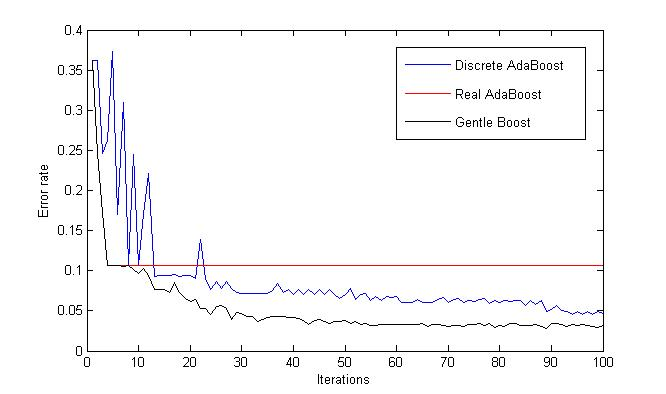
\includegraphics[width=0.7\textwidth]{loss_exp.jpg}
  	\caption{Error rates corresponding to \textsl{Discrete AdaBoost}, \textsl{Real AdaBoost} and \textsl{Gentle AdaBoost}.}
  	\label{loss_exp}
\end{figure}

This loss function is used in some of the most popular boosting algorithms like \textsl{Discrete AdaBoost} or \textsl{Real AdaBoost}; we use it as an example for our model. Firstly the direction descent at $m^{th}$ step $d_m = \nabla_{\overline{F}} Q(\overline{F})\vert_{\overline{F} = \overline{F}_{m-1}} = \left( y_ie^{-y_iF_{m-1}(x_i)}\right)_{i=1:N}$. Following 2(b), we look for $f_m \in \mathcal{Q}_m$ and $c > 0$ which minimize:
\begin{align}
    S(f_m, c) = \sum\limits_{i=1}^N \left( y_ie^{-y_iF_{m-1}(\textbf{x}_i)} - cf_m(\textbf{x}_i)\right)^2 \label{exp_loss_approcher}
\end{align}

If we precise $\mathcal{Q}_m$ so that $f_m(\textbf{x}) \in \{-1, 1\}, \forall \textbf{x}$, we have:
\begin{align}
    S(f_m, c) = Nc^2 + \sum\limits_{i=1}^N e^{-2y_iF_{m-1}(\textbf{x}_i)} - 2c\sum\limits_{i=1}^N e^{-y_iF_{m-1}(\textbf{x}_i)} + c\sum\limits_{i=1}^N e^{-y_iF_{m-1}(\textbf{x}_i)}(y_i - f_m(\textbf{x}_i))^2 \notag
\end{align}
so if we put $w_i = e^{-y_iF_{m-1}(\textbf{x}_i)}$, we have to solve $arg\min\limits_{f_m \in \mathcal{Q}_m} \sum\limits_{i=1}^N w_i(y_i - f_m(\textbf{x}_i))^2$ which is equivalent to classification of $\textbf{x}_i$ using weights $w_i$. The line 2(c) is equivalent to:
\begin{align}
    \beta_m &= arg\min\limits_{\beta \in \mathbb{R}} \sum\limits_{i=1}^N e^{-y_i(F_{m-1}(\textbf{x}_i)+\beta f_m(\textbf{x}_i))} \notag \\
    &= arg\min\limits_{\beta \in \mathbb{R}} \sum\limits_{i=1}^N w_ie^{-\beta y_if_m(\textbf{x}_i)} \notag \\
    &= arg\min\limits_{\beta \in \mathbb{R}} \left( e^{-\beta}\times \sum\limits_{y_i = f_m(\textbf{x}_m)} w_i + e^{\beta}\times \sum\limits_{y_i \neq f_m(\textbf{x}_i)} w_i\right) \notag \\
    &= \dfrac{1}{2}\log\left( \dfrac{\sum\limits_{y_i = f_m(\textbf{x}_i)} w_i}{\sum\limits_{y_i \neq f_m(\textbf{x}_i)} w_i}\right) \notag
\end{align}
we obtain Discrete AdaBoost algorithm described in the table below.

\begin{center}
	\fbox{
	    \parbox{0.9\textwidth}{
	        \textbf{Discrete AdaBoost}\\
	        1. Start with weights $w_i = 1/N, i = 1,...,N$.\\
	        2. Repeat for $m = 1,2,...,M$:\\
	        (a) Fit the classifier $f_m(x) \in \{-1, 1\}$ using weights $w_i$ on the training data.\\
	        (b) Compute $err_m = \mathbb{E}_w \left[ 1(y\neq f_m(\textbf{x}))\right]$, and $\beta_m = \log\left( \dfrac{1-err_m}{err_m}\right)$.\\
	        (c) Set $w_i \leftarrow w_i\times e^{\beta_m\times 1(y_i \neq f_m(\textbf{x}_i))}, i = 1,...,N$, and renormalize $w$.\\
	        3. Output the classifier $sign\left[ \sum\limits_{m=1}^M \beta_mf_m(\textbf{x})\right]$.
	    }
	}
\end{center}

Now we extend the subset $\mathcal{Q}_m$ to contain $f_m$ of real values and not only the functions with discrete values $\{-1, 1\}$. \textsl{Real AdaBoost} is a boosting algorithm that uses such base classifiers. In order to understand this algorithm, we note that \textsl{Real AdaBoost} does not use gradient as the direction of descent $d_m$, but find it directly from an optimization problem. The coefficient of descent $\beta_m$ is taken value $1$. Firstly, $d_m$ is calculated by:
\begin{align}
    d_m = arg\min\limits_{d\in \mathbb{R}^N} Q(\overline{F}_{m-1} + d) = arg\min\limits_{d\in \mathbb{R}^N} \sum\limits_{i=1}^N e^{-y_i(F_{m-1}(\textbf{x}_i) + d^{(i)})} \notag
\end{align}
In order to calculate exactly $d_m$ as an estimate of some added regression function $f_m$'s values, we remark that in $(\textbf{x}_i, y_i)$, there may be many $\textbf{x}_i$ taking a same values, so $(F(\textbf{x}_i))_{i=1:N}$ and then $d_m$ may not be real vectors in $\mathbb{R}^N$. By simplicity, we parameterize $d_m$ by $\textbf{x}$ (which are different values in $(\textbf{x}_i)_{i=1:N}$) and not by $i = 1:N$. We have:
\begin{align}
    d_m(\textbf{x}) = arg\min\limits_{d(\textbf{x}) \in \mathbb{R}} \sum\limits_{\textbf{x}_i = \textbf{x}} e^{-y_i(F_{m-1}(\textbf{x}_i) + d(\textbf{x}))} \notag
\end{align}
We imply that $d_m(\textbf{x}) = \dfrac{1}{2} \log\left( \dfrac{\sum\limits_{\textbf{x}_i = \textbf{x}, y_i = 1} w_i}{\sum\limits_{\textbf{x}_i = \textbf{x}, y_i = -1} w_i}\right)$. We do not use the least-square criterion to find a regression function in $\mathcal{Q}_m$ that approximates $d_m$ (line 2(b) of the Generic Algorithm). Instead, we use a comment that, $d_m(\textbf{x})$ is in fact an empirical estimation of the quantity $\dfrac{1}{2} \log\left( \dfrac{\mathbb{P}_w(y=1\vert \textbf{x})}{\mathbb{P}_w(y=-1\vert \textbf{x})}\right)$ after having trained $\textbf{x}$ and $y$ on training set $(\textbf{x}_i, y_i)_{i=1:N}$ with weights $w_i, i = 1,...,N$. The coefficient $\beta_m$ is taken $1$. We have the following \textsl{Real AdaBoost} algorithm.

\begin{center}
	\fbox{
	    \parbox{0.9\textwidth}{
	        \textbf{Real AdaBoost}\\
	        1. Start with weights $w_i = 1/N, i = 1,...,N$.\\
	        2. Repeat for $m = 1,2,...,M$:\\
	        (a) Fit the classifier to obtain a class probability estimate $p_m(\textbf{x}) = \hat{P}_w(y=1\vert \textbf{x}) \in \left[0, 1\right]$, using weights $w_i$ on the training data.\\
	        (b) Set $f_m(\textbf{x}) = \dfrac{1}{2}\log \dfrac{p_m(\textbf{x})}{1-p_m(\textbf{x})}$.\\
	        (c) Update $w_i \leftarrow w_ie^{-y_if_m(\textbf{x}_i)}$ and renormalize.\\
	        3. Output the classifier $sign\left[ \sum\limits_{m=1}^M f_m(\textbf{x})\right]$.
	    }
	}
\end{center}

The last algorithm that we want to present in this section is \textsl{Gentle AdaBoost}. This algorithm use $\beta_m = 1$ but $d_m$ is not calculated from a direct optimization but from the stepping of Newton-Raphson algorithm. Like in \textsl{Real AdaBoost}, we parameterize $d_m$ not by $i=1:N$ but by $\textbf{x}$ which are the differents values in $(\textbf{x}_i)_{i=1:N}$. We note that the algorithms with such parameterization of $d_m$ is called \textbf{population version}. More precisely,
\begin{align}
    d_m(\textbf{x}) &= -\left( \dfrac{\partial^2 Q}{\partial F(\textbf{x})^2}\right)^{-1}\dfrac{\partial Q}{\partial F(\textbf{x})} \vert_{F(\textbf{x}) = F_{m-1}(\textbf{x})} \notag \\
    &= \dfrac{\sum\limits_{\textbf{x}_i = \textbf{x}} y_ie^{-y_iF(\textbf{x}_i)}}{\sum\limits_{\textbf{x}_i = \textbf{x}} e^{-y_iF(\textbf{x}_i)}} = \dfrac{\sum\limits_{\textbf{x}_i = \textbf{x}} w_iy_i}{\sum\limits_{\textbf{x}_i = \textbf{x}} w_i} \notag
\end{align}
We recognize that $d_m(\textbf{x})$ is in fact an empirical estimation of the quantity $\mathbb{E}_w(y\vert \textbf{x})$; therefore we take $f_m(\textbf{x})$ to be the regression of $y$ to $\textbf{x}$ with weights $w_i$ on the training data. We have the following \textsl{Gentle AdaBoost} algorithm.

\begin{center}
	\fbox{
	    \parbox{0.9\textwidth}{
	        \textbf{Gentle AdaBoost}\\
	        1. Start with weights $w_i = 1/N, i = 1,...,N$.\\
	        2. Repeat for $m = 1,2,...,M$:\\
	        (a) Fit the regression function $f_m(\textbf{x})$ by weighted least-squares of $y_i$ to $\textbf{x}_i$ with weights $w_i$.\\
	        (b) Update $F(\textbf{x}) \leftarrow F(\textbf{x}) + f_m(\textbf{x})$.\\
	        (c) Update $w_i \leftarrow w_ie^{-y_if_m(\textbf{x}_i)}$ and renormalize.\\
	        3. Output the classifier $sign\left[ F(\textbf{x})\right] = sign\left[ \sum\limits_{m=1}^M f_m(\textbf{x})\right]$.
	    }
	}
\end{center}

\textbf{Experiments:} Here we compare the performance of these three algorithms on a same simulated dataset. The dataset is simulated following the following rules: $\textbf{x} \in \mathbb{R}^2$ follows uniform distribution in $(0, 1)^2$, and $y_i = 2*1((\textbf{x}_i^{(1)} - 0.5)^2 + (\textbf{x}_i^{(2)} - 0.5)^2 > 1/6) - 1$. The Bayes error is therefore $0$. We can see that the \textsl{Gentle AdaBoost} obtain the best performance in this experiment. The \textsl{Gentle AdaBoost} corresponds to two-degree optimization in function space (Newton-Raphson algorithm) while the \textsl{Discrete AdaBoost} corresponds to one-degree method. We can link this result to the dominating convergence rate of two-degree methods in numerical optimization.

\subsection{$L(y, F(\textbf{x})) = (y - F(\textbf{x}))^2/2$}
In this section, we will use least-square as the loss function. The updating terms of $F_m$ in the line 2(d) of our generic algorithm will be specifically derived. The least-square loss function is defined as: $L(y, F) = \dfrac{(y-F)^2}{2}$. Now, we can determine the negative gradient, or, the descent direction $d_m = -\dfrac{\partial{Q}}{\partial{\overline{F}}}\vert_{\overline{F} = F_{m-1}} = y - F_{m-1}$. If we apply line search for 2(c), it turns out that $\beta_m = c$. Indeed, with finite data, to do the line search is to find $\beta_m$ such that:
\begin{align}
	\beta_m  &= arg\min\limits_{\beta}\sum_{i=1}^{N}{Q(y_i, F_{m-1}(x_i) + \beta\overline{f_m})} \notag \\
	&= arg\min\limits_{\beta}\sum_{i=1}^{N}{\dfrac{(y_i - F_{m-1}(x_i) - \beta\overline{f_m})^2}{2}}\notag \\
	&= arg\min\limits_{\beta}\sum_{i=1}^{N}{\dfrac{(d_m - \beta\overline{f_m})^2}{2}}\notag \\
	&= arg\min\limits_{\beta}\| d_m - \beta\overline{f_m}\|^2 = c\notag
\end{align}

So, with least-square loss function, the generic algorithm ends up the following LS\_Boost algorithm

\begin{center}
	\fbox{
	    \parbox{0.9\textwidth}{
	        \textbf{Least-Square Boost}\\
		1. Start with $F_0(\textbf{x}) = 0$.\\
		2. Repeat for $m = 1,2,...,M$:\\
		(a) $\overline{y}_i = y_i - F_{m-1}(\textbf{x}_i), i=1:N$\\
		(b) Solve $\left\lbrace f_m, \beta_m\right\rbrace = arg\min\limits_{\overline{f_m}\in \mathcal{Q}_m, \beta\in \mathbb{R}} \| \overline{y} - \beta\overline{f_m}\|^2$.\\
		(c) $F_m(\textbf{x}) = F_{m-1}(\textbf{x}) + \beta_mf_m(\textbf{x})$.\\
		3. Output the classifier $sign\left[ F(\textbf{x})\right]$.
	}
	}
\end{center}


\subsection{$L(y, F(\textbf{x})) = \vert y - F(\textbf{x})\vert$}\label{LAD}
\label{sec:LAD_treeboost}
With $L(y, F(\textbf{x})) = \vert y - F(\textbf{x})\vert$, we choose $d_m^{(i)} = \dfrac{\partial Q}{\partial \overline{F}_i}\vert_{\overline{F} = \overline{F}_{m-1}} = sign(y_i - F_{m-1}(\textbf{x}_i)), \forall i = 1:N$. We can always follow the generic algorithm presented in \ref{boo_fun_sp} with all kinds of base classifiers. Here we discuss on how to adapt regression tree to our boosting algorithm, because it will be the only base classifier used in our experiments.

Firstly, we remark that the coefficient $c > 0$ in the line 2(b) of our generic algorithm does not change fondamentally the properties of regression trees $f_m$; it suffices to get regression tree $f_m$ to approximate the direction $d_m$. A regression tree $f_m$ divide $\mathcal{X}$-space into $K$ disjoint subspace $R_{m,k}$ so that $\bigcup\limits_{k=1}^K R_{m,k} = \mathcal{X}$. For $\textbf{x}$ belonging to each of these areas, $f_m(\textbf{x})$ takes a value $\lambda_{m,k}$. We can rewrite $f_m(\textbf{x}) = \sum\limits_{k=1}^K \lambda_{m,k} 1(\textbf{x}\in R_{m,k})$. The constant $\beta_m$ in the line 2(c) changes these values $\lambda_{m,k}$ by a same way. Another method which gives a better optimization than line 2(c) is to modify all regression values $\lambda_{m,k}$ in this phase and not only the parameter $\beta_m$, that means:
\begin{align}
    \{ \lambda_{m,k}\}_{k=1:K} = arg\min\limits_{\lambda \in \mathbb{R}^K} Q(F_{m-1} + \sum\limits_{k=1}^K \lambda_k 1(\textbf{x} \in R_{m,k})) \notag
\end{align}
This method is clearly more powerful than optimization only on $\beta_m$ and is in fact operated separately in each $R_{m,k}$: For each $k=1:K$,
\begin{align}
    \lambda_{m,k} = arg\min\limits_{\lambda \in \mathbb{R}} \sum\limits_{\textbf{x}_i \in R_{m,k}} L(y_i, F_{m-1}(\textbf{x}_i) + \lambda) \label{opt_LAD_local}
\end{align}
Finally, the areas $R_{m,k}$ are divided accordint to the regression in line 2(b), which tries to approximate $d_m$ by $f_m$ (as explained, we have taken $c = 1$).

For the absolute loss function, according to \eqref{opt_LAD_local}, we have $\lambda_{m,k} = arg\min\limits_{\lambda \in \mathbb{R}} \vert y_i - F_{m-1}(\textbf{x}_i) - \lambda\vert = \text{median} \{y_i - F_{m-1}(\textbf{x}_i)\}_{i, \textbf{x}_i \in R_{m,k}}$, $\forall k=1:K$. We obtain \textsl{LAD TreeBoost} algorithm described below.

\begin{center}
	\fbox{
	    \parbox{0.9\textwidth}{
	        \textbf{LAD TreeBoost}\\
	        1. Start with $F_0(\textbf{x}) = 0$.\\
	        2. Repeat for $m = 1,2,...,M$:\\
	        (a) $\overline{y}_i = sign(y_i - F_{m-1}(\textbf{x}_i)), i = 1:N$.\\
	        (b) $\{R_{m,k}\}_{k=1:K}$ is the $K$-terminal node tree regression of $\overline{y}_i$ on $\textbf{x}_i, i = 1:N$.\\
	        (c) $\lambda_{m,k} = \text{median}\{y_i - F_{m-1}(\textbf{x}_i)\}_{i, \textbf{x}_i \in R_{m,k}}$ for $k=1:K$.\\
	        (d) $F_m(\textbf{x}) = F_{m-1}(\textbf{x}) + \sum\limits_{k=1}^K \lambda_{m,k} 1(\textbf{x} \in R_{m,k})$.\\
	        3. Output the classifier $sign\left[ F(\textbf{x})\right]$.
	    }
	}
\end{center}

\subsection{M-regression loss function}
We consider here the Huber loss function, which is defined as:
\begin{align}
	L(y, F(\textbf{x})) = \left\{
				\begin{array}{cl}
					\frac{(y-F(\textbf{x}))^2}{2} & \quad \text{if $|y-F(\textbf{x})| \leq \delta$}\\
					\delta(|y-F(\textbf{x})|-\delta/2) & \quad \text{if $|y-F(\textbf{x})| > \delta$}\\
				\end{array} 
			\right., \delta\in\mathbb{R}^{+} \notag
\end{align}

<<<<<<< .mine

Then, we have the negative gradient:
\begin{align}
	d_m^{(i)} = -\dfrac{\partial{Q}}{\partial{\overline{F}_i}}\vert_{\overline{F} = F_{m-1}} = \left\{
		\begin{array}{cl}
			y_i-F_{m-1} & \quad \text{if $|y_i-F_{m-1}(\textbf{x}_i)| \leq \delta$}\\
			\delta.\text{sign}(y_i-F_{m-1}(\textbf{x}_i)) & \quad \text{if $|y_i-F_{m-1}(\textbf{x}_i)| > \delta$}\\
		\end{array}
		\right., \forall i = 1:N\notag
\end{align}

As a significant parameter of the loss function, $\delta$ should be chosen considerately. Before going into detail, we should observe that $d_m^{(.)}$ is constrained by $\delta$. The meaning of using $\delta$ here is to remove outliers. Indeed, those points, which have big difference between target output $y$ and estimated output $F_{m-1}(\textbf{x})$, will be excluded from updating process. From now on, we should remark M-Regression's characteristic of resisting to long-tailed error distribution and outliers. The value of $\delta$ will be redetermined iteratively, based on the distribution of residuals $y-F^{*}$, with $F^{*}$ as the true target function. Normally, at $m^{th}$ iteration, we often choose $\delta = \delta_m$ as $\alpha$-quantile of current approximate absolute residual distribution $|y - F_{m-1}|$. Then, the factor is determined by $\delta_m = \text{quantile}_{\alpha}(|y - F_{m-1}|)$.

If we use regression trees as base classifiers, the results in \ref{sec:LAD_treeboost} could be exploited. 
Let's consider $(R_{m,1}, R_{m,2},..., R_{m,K})$ as the partition of $\mathcal{X}$-space, determined by the regression tree at $m^{th}$ iteration. The updating equation then becomes $F_m = F_{m-1} + \sum\limits_{k=1}^{K}{\lambda_{m,k}1(\textbf{x}\in{R_{m,k}})}$ with
\begin{align}
	\lambda_{m,k} =arg\min\limits_{\lambda}\sum\limits_{\textbf{x}_i\in{R_{m,k}}}{L(y_i, F_{m-1}(\textbf{x}_i + \lambda))} \notag
\end{align}

One approximation of $\lambda_{m,k}$ is given in [ref], which requires the median of the current residual $\tilde{r}_{m,k} = median_{\textbf{x}_i\in{R_{m,k}}}(\underbrace{y_i - F_{m-1}(\textbf{x}_i)}_{r_{m-1}(\textbf{x}_i)}), \forall{k}=1:K$. The approximate $\lambda_{m,k}, \forall{k}=1:K$ is then computed by:
\begin{align}
	\lambda_{m,k} = \tilde{r}_{m,k} + \frac{1}{N_{m,k}}\sum_{\textbf{x}_i\in{R_{m,k}}}sign(r_{m-1}(\textbf{x}_i) - \tilde{r}_{m,k}) \cdot min(\delta_m, |r_{m-1}(\textbf{x}_i) - \tilde{r}_{m,k}|) \notag
\end{align}

Now, we obtain an boosting algorithm using regression tree and Huber loss function, which is called M-TreeBoost

\begin{center}
	\fbox{
	    \parbox{0.9\textwidth}{
	        \textbf{M-TreeBoost}\\
	1. Start with $F_0(\textbf{x}) = 0$.\\
	2. Repeat for $m = 1,2,...,M$:\\
	(a) $r_{m-1}(\textbf{x}_i) = y_i - F_{m-1}(\textbf{x}_i), \forall i=1:N$.\\
	(b) $\delta_m =\text{quantile}_\alpha{|r_{m-1}(\textbf{x}_i)|}, \forall i=1:N$.\\
	(c) $\overline{y}_i = \left\{
		\begin{array}{cl}
			y_i-F_{m-1}(\textbf{x}_i) & \quad \text{if} |y_i-F_{m-1}(\textbf{x}_i)| \leq \delta_m \\
			\delta_m.\text{sign}(y_i-F_{m-1}(\textbf{x}_i)) & \quad \text{if} |y_i-F_{m-1}(\textbf{x}_i)| > \delta_m\\
		\end{array}\right.$\\
	(d) $\{R_{m,k}\}_{k=1:K}$ is the $K$-terminal node tree regression of $\overline{y}_i$ on $\textbf{x}_i, i = 1:N$.\\
	(e) $\tilde{r}_{m,k} = median_{\textbf{x}_i\in{R_{m,k}}}({r_{m-1}(\textbf{x}_i)})$\\
	(f) $\lambda_{m,k} = \tilde{r}_{m,k} + \frac{1}{N_{m,k}}\sum_{\textbf{x}_i\in{R_{m,k}}}sign(r_{m-1}(\textbf{x}_i) - \tilde{r}_{m,k}) \cdot min(\delta_m, |r_{m-1}(\textbf{x}_i) - \tilde{r}_{m,k}|)$.\\
	(g) $F_m(\textbf{x}) = F_{m-1}(\textbf{x}) + \sum\limits_{k=1}^K \lambda_{m,k} 1(\textbf{x} \in R_{m,k})$.\\
	3. Output the classifier $sign\left[ F(\textbf{x})\right]$.
	}
	}
\end{center}


\subsection{Negative Binomial log-likelihood loss function}

\begin{figure}[ht]\centering
  	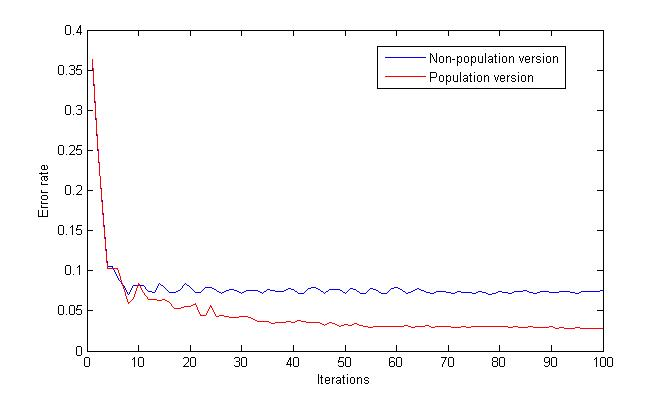
\includegraphics[width=0.7\textwidth]{comp_pop_nonPop.jpg}
  	\caption{Comparison of the performance of population and non-population version of \textsl{Logit Boost} algorithm on simulated data.}
  	\label{comp_pop_nonPop}
\end{figure}

The binomial log-likelihood loss function is $L(y, F(\textbf{x})) = \log\left( 1 + e^{2F(\textbf{x})}\right) - 2y^{*}F(\textbf{x})$ in which $y^{*} = \dfrac{y+1}{2}$. In Bernouilli model, the probability that $y^{*}$ taking value $1$ is $p(\textbf{x}) = \dfrac{e^{F(\textbf{x})}}{e^{F(\textbf{x})} + e^{-F(\textbf{x})}}$. The negative log-likelihood is calculated by:
\begin{align}
    L(y, F(\textbf{x})) &= -y^{*}\log p(\textbf{x}) - (1-y^{*})\log(1-p(\textbf{x})) \notag \\
    &= \log\left( 1+e^{2F(\textbf{x})}\right) + y^{*}\log \dfrac{1+e^{-2F(\textbf{x})}}{1+e^{2F(\textbf{x})}} \notag
\end{align}
We replace the last term simply by $-2y^{*}F(\textbf{x})$, and obtain the loss function above.

The direction of descent $d_m$ is taken to be the Newton-Raphson steps in the \textbf{population version} ($d_m$ is parameterized by $\textbf{x}$). By denoting $p_m(\textbf{x}_i) = \dfrac{e^{F_{m-1}(\textbf{x}_i)}}{e^{F_{m-1}(\textbf{x}_i)} + e^{-F_{m-1}(\textbf{x}_i)}}$ and by ignoring some multiplying constants in \textsl{Hessian} matrix, we have:
\begin{align}
    d_m(\textbf{x}) &= -\left( \dfrac{\partial^2 Q}{\partial F(\textbf{x})^2}\right)^{-1}\dfrac{\partial Q}{\partial F(\textbf{x})} \vert_{F = F_{m-1}} \notag \\
    &= \dfrac{\sum\limits_{\textbf{x}_i = \textbf{x}} (y_i^{*} - p_m(\textbf{x}_i))}{\sum\limits_{\textbf{x}_i = \textbf{x}} p_m(\textbf{x}_i)(1 - p_m(\textbf{x}_i))} \notag
\end{align}
If we put $w_i = p_m(\textbf{x}_i)(1-p_m(\textbf{x}_i))$ on the training data, we have $d_m(\textbf{x}) = \dfrac{\sum\limits_{\textbf{x}_i = \textbf{x}} \dfrac{y_i^{*} - p_m(\textbf{x}_i)}{p_m(\textbf{x}_i)(1 - p_m(\textbf{x}_i))}w_i}{\sum\limits_{\textbf{x}_i = \textbf{x}} w_i}$. We recognize that this is an empirical estimation of the quantity $\mathbb{E}_w \left[ \dfrac{y^{*} - p(\textbf{x})}{p(\textbf{x})(1 - p(\textbf{x}))}\vert \textbf{x}\right]$. The coefficient $\beta_m$ is taken value $\dfrac{1}{2}$. Then we have the following population version of \textsl{Logit Boost} algorithm.

\begin{center}
	\fbox{
	    \parbox{0.9\textwidth}{
	        \textbf{Logit Boost (2 classes)}\\
	        1. Start with weights $w_i = 1/N$, $F(\textbf{x}) = 0$ and probability estimates $p(\textbf{x}_i) = 1/2$.\\
	        2. Repeat for $m = 1,2,...,M$:\\
	        (a) Compute $z_i = \dfrac{y_i^{*} - p(\textbf{x}_i)}{p(\textbf{x}_i)(1 - p(\textbf{x}_i))}$ and $w_i = p(\textbf{x}_i)(1 - p(\textbf{x}_i))$.\\
	        (b) Fit the function $f_m(\textbf{x})$ by a weighted least-squares regression of $z_i$ to $\textbf{x}_i$ using weights $w_i$.\\
	        (c) Update $F(\textbf{x}) \leftarrow F(\textbf{x}) + \dfrac{1}{2}f_m(\textbf{x})$, and $p(\textbf{x}) = \dfrac{e^{F(\textbf{x})}}{e^{F(\textbf{x})} + e^{-F(\textbf{x})}}$.\\
	        3. Output the classifier $sign\left[ F(\textbf{x})\right] = sign\left[ F(\textbf{x})\right]$.
	    }
	}
\end{center}

In the derivation of this \textsl{Logit Boost} algorithm, we comment that although $\textbf{x}_i = \textbf{x}$, the quantity $p_m(\textbf{x}_i)(1 - p_m(\textbf{x}_i))$ is not constant. Indeed, in our implementation $p_m(\textbf{x}_i)$ depends on $F_{m-1}(\textbf{x}_i)$ with parameterization by $i=1:N$ and not by $\textbf{x}$. The interpretation of the population version is, although all $F_m$ and $f_m$ is calculated on $\{ \textbf{x}_i\}_{i=1:N}$, their right parameterization in function space is by $\textbf{x} \in \mathcal{X}$ and not by $i=1:N$. The vector $d_m$ parameterized by $\textbf{x} \in \mathcal{X}$ may be easier to be used in regression of function $f_m$. This is an advantage of the point of view that considers boosting as an optimization in the function space.

\textbf{Comparison between population and non-population versions.} There exists a \textbf{non-population version} of \textsl{Logit Boost} that consists on doing regression of $f_m$ \textbf{without weights} $w$. We can derive it by parameterizing vector $d_m$ by $d_m^{(i)}\vert_{i=1:N}$. We use the same simulated dataset than one used in \ref{exp_loss_part} to compare these two versions. The results in Fig. \ref{comp_pop_nonPop} prove the good performance of population version compared to the non-population one.

\subsection{$L(y, F(\textbf{x})) = \log(1+e^{-2yF(\textbf{x})})$}
For the negative binomial log-likelihood loss function $L(y, F) = log(1+e^{-2yF})$, we obtain the descent direction $d_m = -\dfrac{\partial{Q}}{\partial{\overline{F}}}\vert_{\overline{F} = F_{m-1}} = \dfrac{2y}{1+e^{2yF_{m-1}}}$. If regression trees are used as base classifiers, we can also inherit results from \ref{sec:LAD_treeboost}, in which the $\lambda_{m,k}$ is now approximated as:
\begin{align}
	\lambda_{m,k} = \frac{\sum\limits_{\textbf{x}_i\in{R_{m,k}}}d_{m}^{(i)}}{\sum\limits_{\textbf{x}_i\in{R_{m,k}}}|d_{m}^{(i)}|(2 - |d_{m}^{(i)}|)} \notag
\end{align}
And, the boosting algorithm is described as in Algorithm \ref{algo:l2_treeboost}

\begin{center}
	\fbox{
	    \parbox{0.9\textwidth}{
	        \textbf{L2-TreeBoost}\\
	1. Start with $F_0(\textbf{x}) = 0$.\\
	2. Repeat for $m = 1,2,...,M$:\\
	(a) $\overline{y}_i = \dfrac{2y_i}{1+e^{2y_iF(\textbf{x}_i)}}$.\\
	(b)$\{R_{m,k}\}_{k=1:K}$ is the $K$-terminal node tree regression of $\overline{y}_i$ on $\textbf{x}_i, i = 1:N$.\\
	(c) $\lambda_{m,k} = \dfrac{\sum\limits_{\textbf{x}_i\in{R_{m,k}}}\overline{y}_i}{\sum\limits_{\textbf{x}_i\in{R_{m,k}}}|\overline{y}_i|(2 - |\overline{y}_i|)}$\\
	(d) $F_m(\textbf{x}) = F_{m-1}(\textbf{x}) + \sum\limits_{k=1}^K \lambda_{m,k} 1(\textbf{x} \in R_{m,k})$.\\
	3. Output the classifier $sign\left[ F(\textbf{x})\right]$.
	}
	}
\end{center}

\section{Multi-class classification and some generalizations}
In this part, we present some generalizations of two-class classification algorithms to the case of multi-classes. In a multi-class classification problem, there are $J > 2$ labels for each line of explanatory variables $\textbf{x}$, denoted by $1,2,...,J$. The response variable $y$ is no longer a vector $\{y_i\}_{i=1:N}$ but a matrix $\{y_{i,j}\}_{1 \leq i \leq N, 1\leq j \leq J}$ defined by:
\begin{align}
    y_{i,j} = \left\lbrace
    \begin{array}{l l}
    	1 & \quad \text{ if label of $\textbf{x}_i$ is $j$,}\\
    	-1 & \quad \text{ if otherwsise}\\
	\end{array} \right. \notag
\end{align}
If we combine the explanatory variables $\textbf{x}$ with each column $y(:, j)$ of $y$, we will obtain $J$ separate two-class classification problems. The algorithms for multi-class case will be based on these $J$ problems that we have tried to resolve in the precedent parts of this report.

Another advantage of this representation of $y$ as a matrix $N\times J$ rather than as a $N$-vector $\in \{1,2,...,J\}^N$ is that we can use it (or some of its variants) to solve more general problems. Schapire, R.E. \& Singer, Y. in \cite{SchaAndSin1998} discussed about some of these generalizations, for example multi-labels problem (in which each $\textbf{x}$-data can corresponds to more than one labels), and label-ranking problem (in which we try to assess a rank on all labels so that the first one is the most likely to be a label of data $\textbf{x}$). We also realize that the methods presented below can be adapted to resolve multi-label problems, because that only consists on deciding value of $y_{i,j}$ for $i=1,...,N$ and $j=1,...,J$ which is also the goal of multi-class problem. However, in scope of this report, we restrict our discussion inside the multi-single class framework.

\subsection{A traditional approach}
\begin{figure}[ht]\centering
  	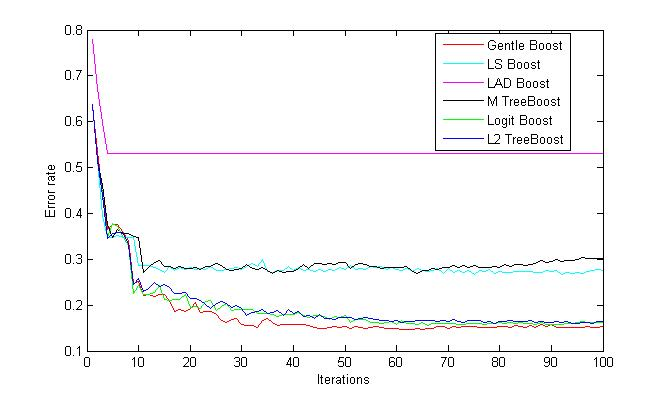
\includegraphics[width=0.7\textwidth]{comp_MH.jpg}
  	\caption{Comparison of the performances of \textsl{AdaBoost.MH} using $6$ two-class boosting methods, experiments on simulated data with $0 \%$ Bayes error.}
  	\label{comp_MH}
\end{figure}

\begin{figure}[ht]\centering
  	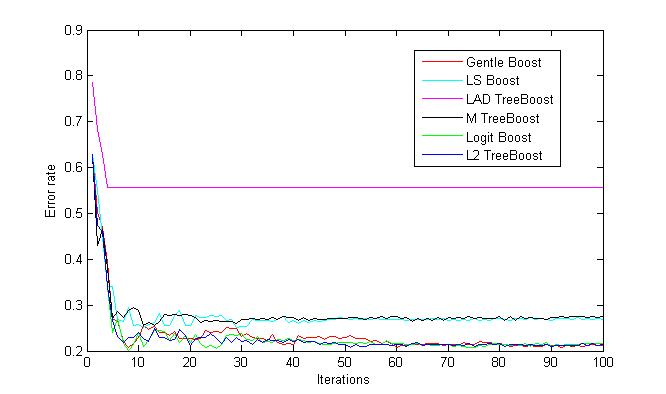
\includegraphics[width=0.7\textwidth]{comp_MH1.jpg}
  	\caption{Comparison of the performances of \textsl{AdaBoost.MH} using $6$ two-class boosting methods, experiments on simulated data with $5 \%$ Bayes error.}
  	\label{comp_MH1}
\end{figure}

\begin{figure}[ht]\centering
  	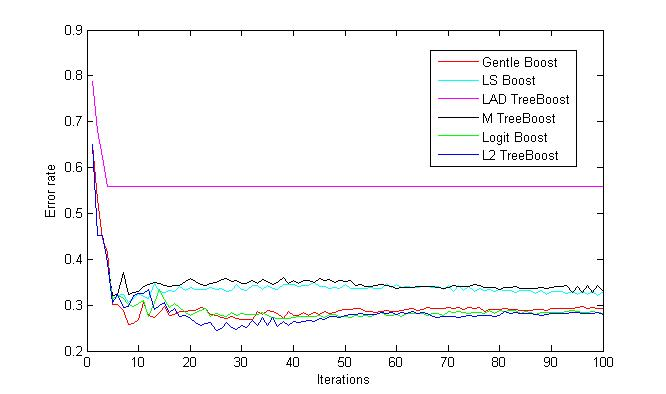
\includegraphics[width=0.7\textwidth]{comp_MH2.jpg}
  	\caption{Comparison of the performances of \textsl{AdaBoost.MH} using $6$ two-class boosting methods, experiments on simulated data with $10 \%$ Bayes error.}
  	\label{comp_MH2}
\end{figure}

The \textsl{One-Against-All} strategy consists on resolve these $J$ classification problems (described above) separately, then for each data $\textbf{x}_i$, we choose the result of the problem in which the score of $\textbf{x}$ is the highest. The \textsl{AdaBoost.MH} algorithm is formalized in the following table.

\begin{center}
	\fbox{
	    \parbox{0.9\textwidth}{
	        \textbf{AdaBoost.MH for multi classes}\\
	        1. Construct response variables $y$ under suitable form ($N\times J$-matrix) using \textsl{One-Agaisnt-All} strategy.\\
	        2. For $j=1,...,J$, we output a boosting classifier $F_j$ for problem $P_j$.\\
	        3. Label of $\textbf{x} = arg\max\limits_{1\leq j \leq J} F_j(\textbf{x})$.
	    }
	}
\end{center}

\textbf{Experiments:} We can use all two-class boosting methods in the line $2$ of the algorithm. Here we use successively \textsl{GentleBoost}, \textsl{LS Boost}, \textsl{LAD TreeBoost}, \textsl{M TreeBoost}, \textsl{Logit Boost} and \textsl{L2 TreeBoost} and compare their performance in multi-class framework on simulated data. The data of $J$ classes is simulated following the rules: $\textbf{x}_i$ is chosen uniformly in $\left[ 0, 1\right]^2$, $r_i^2$ is the squared distance from $\textbf{x}_i$ to $(1/2, 1/2)$, $\textbf{x}_i$ corresponds to label $j$ if $\dfrac{j-1}{J} \leq \pi r_i^2 < \dfrac{j}{J}, j = 1,2,...,J$. We take $J = 4$ and the Bayes error to be $0 \%$, $5 \%$ and $10 \%$. The results in Fig. \ref{comp_MH} , Fig. \ref{comp_MH1} and Fig. \ref{comp_MH2} show that the performance of \textsl{AdaBoost.MH} is the best when combining \textsl{AdaBoost.MH} with \textsl{Gentle Boost}, \textsl{Logit Boost} and \textsl{L2 TreeBoost}.

\subsection{Some generalization of two-class algorithms}

\begin{figure}[ht]\centering
  	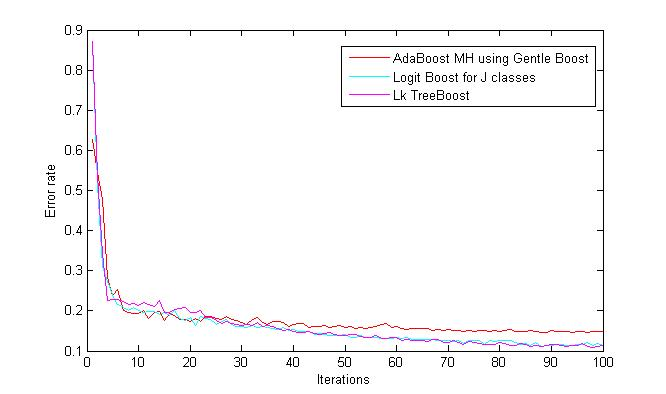
\includegraphics[width=0.7\textwidth]{multi_comp0.jpg}
  	\caption{Multi-class classification on simulated data, $J = 4$, Bayes error $0\%$.}
  	\label{multi_comp0}
\end{figure}

\begin{figure}[ht]\centering
  	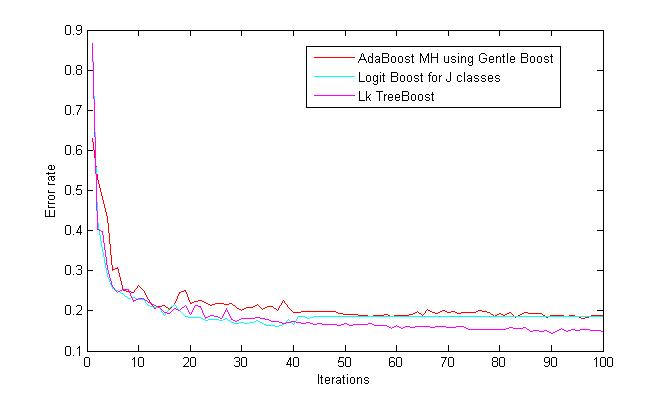
\includegraphics[width=0.7\textwidth]{multi_comp1.jpg}
  	\caption{Multi-class classification on simulated data, $J = 4$, Bayes error $5\%$.}
  	\label{multi_comp1}
\end{figure}

\begin{figure}[ht]\centering
  	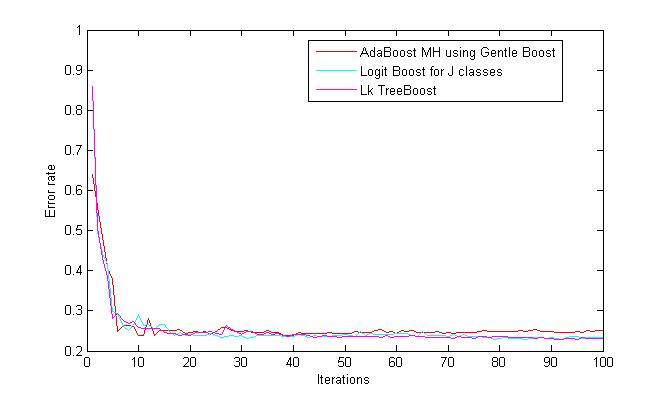
\includegraphics[width=0.7\textwidth]{multi_comp2.jpg}
  	\caption{Multi-class classification on simulated data, $J = 4$, Bayes error $10\%$.}
  	\label{multi_comp2}
\end{figure}

\begin{figure}[ht]\centering
  	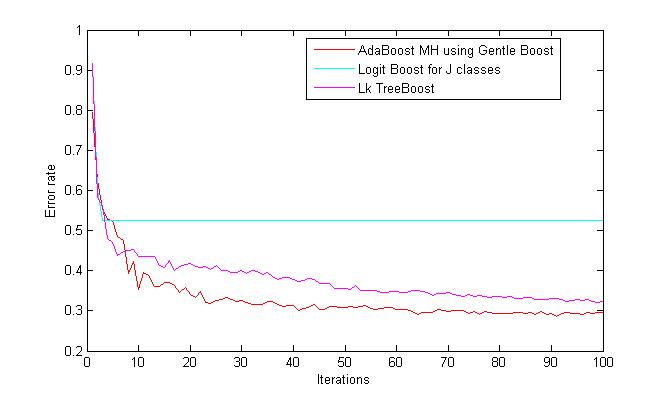
\includegraphics[width=0.7\textwidth]{multi_comp3.jpg}
  	\caption{Multi-class classification on simulated data, $J = 6$, Bayes error $0\%$.}
  	\label{multi_comp3}
\end{figure}

Some of two-class algorithms have their generalizations in multi-class case. In this section, we present the usage of the negative Binomial likelihood loss function in multi-class framework.
\begin{align}
    L(y, F(\textbf{x})) = -\sum\limits_{j=1}^J y_j^{*}\log p_j(\textbf{x}) \notag
\end{align}
in which $p_j(\textbf{x}) = \dfrac{e^{F_j(\textbf{x})}}{\sum\limits_{l=1}^J e^{F_l(\textbf{x})}}, j = 1:J$.

We derive the multi-class version of \textsl{Logit Boost} similarly as in two-class case in taking $d_m$ to be Newton-Raphson steps by a \textbf{population version} way (parameterize $d_m$ by $\textbf{x}$). If instead, we only take $d_m$ to be the gradient in a parameterization by $i$ (\textbf{non-population version}) and then process the line-search via regression trees like what we have explained in \ref{LAD}, we obtain \textsl{Lk TreeBoost} algorithm. These two algorithms are summarized below.

\begin{center}
	\fbox{
	    \parbox{0.9\textwidth}{
	        \textbf{LogitBoost for $J$ classes}\\
	        1. Start with weights $w_{ij} = 1/N, i = 1:N, j = 1:J, F_j(\textbf{x}) = 0$ and $p_j(\textbf{x}) = 1/J, \forall j = 1:J$.\\
	        2. Repeat for $m = 1,2,...,M$:\\
	        (a) Repeat for $j=1,...,J$:\\
	        i. Compute $z_{ij} = \dfrac{y_{ij}^{*} - p_j(\textbf{x}_i)}{p_j(\textbf{x}_i)(1 - p_j(\textbf{x}_i))}$ and $w_{ij} = p_j(\textbf{x}_i)(1 - p_j(\textbf{x}_i))$.\\
	        ii. Fit the function $f_{mj}(\textbf{x})$ by a weighted least-squares regression of $z_{ij}$ to $\textbf{x}_i$ with weights $w_{ij}$.\\
	        (b) Set $f_{mj}(\textbf{x}) \leftarrow \dfrac{J-1}{J}\left( f_{mj}(\textbf{x}) - \dfrac{1}{J}\sum\limits_{k=1}^J f_{mk}(\textbf{x})\right)$.\\
	        (c) Update $p_j(\textbf{x})$ via $F_k(\textbf{x}), k = 1:J$.\\
	        3. Output the classifier $arg\max\limits_{j=1:J} F_j(\textbf{x})$.
	    }
	}
\end{center}

\begin{center}
	\fbox{
	    \parbox{0.9\textwidth}{
	        \textbf{Lk TreeBoost for $J$ classes}\\
	        1. Start with $F_j(\textbf{x}) = 0, \forall j = 1:J$.\\
	        2. Repeat for $m = 1,2,...,M$:\\
	        (a) Update $p_j(\textbf{x})$ via $F_j(\textbf{x}), j = 1:J$.\\
	        (b) Repeat for $j=1,...,J$:\\
	        i. Compute $z_{ij} = y_{ij}^{*} - p_j(\textbf{x}_i)$.\\
	        ii. Fit regression tree $\{ R_{kjm}\}_{k=1:K}$ a $K$-terminal node from the training $\{ z_{ij}, x_i\}_{i=1:N}$.\\
	        iii. Take $\lambda_{kjm} = \dfrac{J-1}{J} \dfrac{\sum\limits_{\textbf{x}_i \in R_{kjm}} z_{ij}}{\sum\limits_{\textbf{x}_i \in R_{kjm}} \vert z_{ij}\vert (1 - \vert z_{ij}\vert)}$, $k = 1:K$.\\
	        iv. $F_{jm}(\textbf{x}) = F_{j,m-1}(\textbf{x}) + \sum\limits_{k=1}^K \lambda_{kjm} 1(\textbf{x} \in R_{kjm})$.\\
	        3. Output the classifier $ arg\max\limits_{j=1:J} F_j(\textbf{x})$.
	    }
	}
\end{center}

\textbf{Experiments:} We use the same simulated multi-class dataset with $J = 4$ and Bayes error is $0\%$, $5\%$ and $10\%$. The results are shown in Fig. \ref{multi_comp0}, \ref{multi_comp1} and \ref{multi_comp2}. With $J=4$, we see that the two generalizations of negative binomial loss function algorithms in multi-class case perform better than all versions of \textsl{AdaBoost MH}. But an disadvantage of \textsl{Logit Boost for J classes}, as mentioned in \cite{boost} and \cite{trebst}, is the numerical instability when one of weights $w(\textbf{x}) = p(\textbf{x})(1 - p(\textbf{x}))$ tends to zero. Indeed, when we try with $J=6$, the result in Fig. \ref{multi_comp3} shows that \textsl{Logit Boost} encounters a numerical problem. In this experiment, \textsl{AdaBoost MH} performs the best among these three algorithms.

\section{Experiments}

\subsection{Experiments with simulated data}

\subsection{Experiments with real data}

\section{Conclusion}

\begin{thebibliography}{9999}%\enlargethispage{\baselineskip}
\bibitem[1]{boost}Friedman, J., Hastie, T. \& Tibshirani, R. \textsl{Additive Logistic Regression: a Statistical View of Boosting}, 2000.

\bibitem[2]{trebst}Friedman, J. \textsl{Greedy Function Approximation: A Gradient Boosting Machine}, IMS 1999 Reitz Lecture, 2001.

\bibitem[3]{SchaAndSin1998}Schapire, R.E. \& Singer, Y. \textsl{Improved Boosting Algorithms: Using Confidence-rated Predictions}, 1998.

\end{thebibliography}

\end{document}